\documentclass{article}
\usepackage[utf8]{inputenc}

\title{Modifying the Least Significant Bit (LSB) Stenography Method In Images to Increase Data Volume Density}
\author{Anish Sachdeva}
\date{November 2020}
\documentclass[titlepage]{article}

\usepackage{natbib}
\usepackage{graphicx}
\usepackage{algorithm}
\usepackage{algorithmic}
\usepackage[utf8]{inputenc}
\usepackage[top=2cm, bottom = 2cm, left=1.5cm, right=1.5cm ]{geometry}
\usepackage{amsfonts, amsmath, amssymb}
\usepackage[none]{hyphenat}
\usepackage{fancyhdr}
\usepackage{float}
\usepackage[nottoc, notlot, notlof]{tocbibind}
\usepackage{hyperref}
\usepackage{multicol}
\usepackage{subfig}
\usepackage{amsmath,amsfonts,amssymb,amsthm}
\usepackage{mathtools}
\usepackage{commath}
\usepackage[sc,osf]{mathpazo}
\usepackage{relsize}
\usepackage{xcolor}
\usepackage[colorlinks]{hyperref}

\pagestyle{fancy}
\fancyhead{}
\fancyfoot{}
\fancyhead[R]{\slshape }
\fancyfoot[c]{\thepage}
\renewcommand{\headrulewidth}{0.5pt}
\renewcommand{\footrulewidth}{0.5pt}

%This command is used to set the indentation of a paragraph
\parindent 0ex
\setlength{\parindent}{0em}
\renewcommand{\baselinestretch}{1.1}

\begin{document}

\begin{titlepage}
\begin{center}
\vspace*{1cm}
\Large{\textbf {Partial Differential Equations (MC-$406$)}}\\
\vfill
\line(1,0){400}\\[1mm]
\huge{\textbf{A Novel a-Posteriori Approach For Eliminating Degradation In Images Caused By Point Spread Functions (PSF) and Restoring Images To Original State}}\\[3mm]
\Large{\textbf{Delhi Technological University}}\\[1mm]
\line(1,0){400}

\vfill  

\includegraphics[height=6cm]{assets/dtu.png}
\vfill

Anish Sachdeva \\
DTU / 2K16 / MC / 13 \\
\end{center}
\end{titlepage}

%Contents Page
\tableofcontents
\thispagestyle{empty}
\clearpage

\clearpage
\setcounter{page}{1}
\section{Acknowledgements}
I would like to express a special thanks of gratitude towards my teacher Prof Dr. Aditya Kaushik of the Mathematics Department (MC) of the Delhi Technological University (DTU) to grant me this amazing opportunity to work on a novel research idea. \\

This project aims to create a novel technique for deblurring of images using a-posteriori method for removing the Point Spread Functions (PSF) that caused image blurring in the original sharp Image. This project mainly pertains in the field of Computer Vision, and I received this idea and initial motivation from Dr. Aditya Kaushik. He gave me countless suggestions throughout the project and also the underlying idea of how this might be accomplished. I thank him for all the suggestions, motivation and many hours of brainstorming so that we could formulate the basis of this project.\\

Lastly I would also take this opportunity to thank my parents and friends who helped me when I was finalizing this project and helped me complete this within the limited time frame.

\clearpage
\section{Abstract}
The development of visual information data forhuman logic and processing for visual data for independent machine perception are the main important areas that have triggered the interest in image processing subject long ago. Image restoration process refers to elimination or minimization{\color{white} :} of degradations in an image. \cite{19} \\

The process of image restoration includes deblurring of images which are degraded by the various limitations of environment, camera sensor, non-linearity’s and noise due to camera sensors or correction of geometric distortion. Image deblurring/deconvolution is a process of recovering the original image from a degraded image. \cite{21} \\

Point spread function (PSF) is a function which causes the degradation of images also called as the blur kernel or degradation function. The light or electromagnetic waves that we intend to capture propagates from a point source. The light spreads due to environmental or imaging system reasons thus reducing the quality of imaging system. This problem is ill conditioned by nature. We propose a method where we use maximum a posterior approach and also use the information in the spectrum of the image to deblur the image. The proposed method is robust and is able to handle a variety of blurs.

\clearpage
\section{Introduction}
Human vision information is the most trusted source of information compared to other data acquisition done by the human body. An image is a generic container of any visual information. The procedure of retrieval and analysis of the visual information by a digital device is called digital image processing. The development of visual information for human logic and processing of visual data for independent machine perception are the main important areas that had triggered the interest in image processing subject long ago \cite{gonzalez-woods}. \\

In fact, when a physical process generates an image, the energy radiated by the source is proportional to its intensity. Hence, the final image, $i(x,y)$, is not zero and finite \cite{jain-anil}, i.e., 

\begin{equation}
    i(x, y) \in \mathbb{Z}
\end{equation} \\

where $\mathbb{Z}$ represents a finite set of integers and $x$, $y$ shows spatial coordinates. Hence, an image is expounded as a two dimensional light intensity function, $i(x, y)$, and the numeric value of $i$, at any given point $(x; y)$ will be corresponding to the brightness of the image at that given point \cite{jain-anil}. A digital image can be expressed as a matrix. Its row and column indices will indicate point in the image. The analogous matrix element can be known as picture element. Its pixel value represents the intensity at that point in the matrix. The input for digital image processing is always an image and the output of it would be an image and some relevant information gathered on function application on the given image. \\

Following are the methods used as techniques of digital image processing \cite{gonzalez-woods}:
\begin{enumerate}
    \item Image Representation / Modeling
    \item Image Enhancement
    \item Image Restoration
    \item Image Analysis
    \item Image Reconstruction
    \item Image Data Compression
\end{enumerate}

\begin{figure}[ht]
    \centering
    \includegraphics{intro/blur-model.PNG}
    \caption{Blur Model}
    \label{fig:blur-model}
\end{figure}

The digital image processing technique followed in this thesis is image restoration. A lot of research has been done in the field of image restoration but lot still needs to be done. Image restoration is a very wide area in image processing hence a part of it has been focused in this thesis that is reconstruction of the true image and blur estimation. 

\subsection{Challenges}
Illumination and reflecting components are the major components which characterizes an image. Apart from these major components an image formation will also depend on the attributes of the object being photographed, environmental conditions at the time of photograph taken and the imaging devices being used. All these components produce an bad effect during image acquisition \cite{22} and results in production of a degraded image, $c$. The process of recovering the actual image from the degraded image is the objective of image restoration. The function causing the degradation in the image, $d_f$ is known as blur. The noise that gets added in the image is also regarded as another source of degradation. Thus the image degradation model can be represented as, 

\begin{equation}
    c = d_f \cdot i + \eta
\end{equation}

We have $c$ (degraded image), some information about the degradation function (blur) $d_f$, and some information about the noise $\eta$. The goal of restoration is to get an estimate of the original (actual) image. The estimate, $\hat{\iota}$, is desired to be as close as possible to the original image. In fact the more the information we have about $d_f$ and $\hat{\iota}$, the more accurate will be the estimation. Figure 1.1 shows the degradation of image and image restoration process. \\

Image restoration process refers to elimination or minimization of degradation in an image. The process of image restoration includes deblurring of images which are degraded by the various limitations of camera sensor, environment, correction of geometric distortion or non-linearity’s and noise due to camera sensors. \\

Image restoration gained importance in the engineering field in the area of astronomical applications. The air has different composition and density at different levels and thus the refractive index is also different. This caused blurred images captured at the ground \cite{jiang-ming}.The large difference in the speeds of space craft and the camera shutter caused motion blur in the images captures of earth and planets. Also medical imaging has a lot of degradations so restoration becomes a crucial part. Visual media has not used the technique to the best of its ability but old movies and videos restoration is an interesting application of image restoration. Image restoration has vast applications in the field of aviation and surveillance and many more applications needs to be explored.

\subsection{Target Definition}
Image deconvolution is a process of recovering the original image from a degraded image \cite{21}. There are two types of image deconvolution, first is the blind image deconvolution and second is{\color{white} j} the non{\color{white} j} blind{\color{white} j} image{\color{white} j} deconvolution{\color{white} j}. Blind{\color{white} j} image{\color{white} j} deconvolution{\color{white} j} is{\color{white} j} a{\color{white} j} process{\color{white} j} of{\color{white} j} deconvolution in which both{\color{white} j} the{\color{white} j} actual image{\color{white} j} and{\color{white} j} the{\color{white} j} degradation function is unknown and only the degraded image is known \cite{23}. Non blind image deconvolution is a process of deconvolution in which we have the knowledge of the degradation function ( blur function / blur kernel / point spread function).  \\

The revival process or recovery process are of two types: 
\begin{enumerate}
    \item Non Blind Restoration
    \item Blind Image Restoration
\end{enumerate}

The first type non blind restoration technique includes that utilizes some knowledge about the blur kernel during revival of the image while the second type blind image restoration technique tries to estimate both{\color{white} j} the{\color{white} j} original image{\color{white} j} and{\color{white} j} the{\color{white} j} degradation (blur{\color{white} j}) from{\color{white} j} the{\color{white} j} degraded{\color{white} j}/blurred image{\color{white} j}, without any knowledge of the imaging system. In the non blind restoration technique, the blur kernel or degradation function{\color{white} j} is{\color{white} j} given{\color{white} j} and{\color{white} j} the{\color{white} j} degradation{\color{white} j}/convolution process{\color{white} j} is{\color{white} j} reverted using{\color{white} j} known restoration algorithms. In the second type that is blind image deconvolution, the degraded image $c(x, y)${\color{white} j}, is{\color{white} j} expected to{\color{white} j} be{\color{white} j} a two{\color{white} j} dimensional{\color{white} j} convolution{\color{white} j} of{\color{white} j} the{\color{white} j} actual{\color{white} j} image{\color{white} j} $i(x, y)${\color{white} j} with{\color{white} j} the blur kernel(degradation function), also known as point spread function (PSF), $d(x; y)$. The relation between the discussed parameters is given by:

\begin{equation}
    c(x, y) = i(x, y) \cdot d(x, y) 
\end{equation}

The{\color{white} j} reconstruction{\color{white} j} of{\color{white} j} the{\color{white} j} original true{\color{white} j} image{\color{white} j} requires{\color{white} j} the{\color{white} j} knowledge of{\color{white} j} blur kernel (PSF{\color{white} j}) and its deconvolution with the degraded(blurred) image. Many researchers have worked and explored the area of image deconvolution but still it is a crucial problem for researches. 

\subsection{Motivation{\color{white} j} For{\color{white} j} Blind{\color{white} j} Image{\color{white} j} Deblurring}
In spite of being a difficult problem, the blind image deconvolution has enjoyed much wide application areas in most of the practical scenarios. The major motivations behind blind image deconvolution can be focused as: 

\begin{enumerate}
    \item Use of high cost adaptive-optics systems to overcome the blurring problem in astronomical imaging is impractical for analyzing some observation. Instead the blind deconvolution is cheapest way to retrieve the relevant information from the degraded image as a post-processing technique. 
    
    \item Some application area such as medical imaging rely on high image quality for close diagnosis, like X-ray imaging, which in turn demands for increased incident X-ray beams intensity. But practically, this is hazardous for patient's health and hence blurring is inevitable. Hence, BID is used to tackle with the degradation.
    
    \item Instant deblurring cannot be done by predetermining certain PSF in real-time applications such as video-conferencing. Also, on-line degradation determining technique is error prone and create artifacts in restored image.
    
    \item Lastly, but not least, to predetermine any information about any scenario is practically either too costly, or dangerous and sometimes mostly impossible. Also, the degradation specified is not necessary true for deblurring. Hence, blind approach is adopted to solve the problem. 
\end{enumerate}


\subsection{Deblurring Characteristics}
Blind deconvolution problem is based on some assumptions. The problem of blind deconvolution of image has few characteristics as listed below:- 

\begin{enumerate}
    \item The signals that convolve to form the degraded image that is the original image and the blur kernel (PSF) are irreducible \cite{jiang-ming}. It is important to have this characteristic as if the degraded image is a resultant of more than two independent components then the deconvolution is ambiguous. If true image $i(x, y) = i_{1}(x, y) \cdot i_{2}(x,y)$ and the blur kernel (PSF), $d(x, y) = d_{1}(x, y) \cdot d_{2}(x, y)$, then
    
    \begin{equation}
        c(x, y) = i_{1}(x, y)\cdot i_{2}(x, y) \cdot d_{1}(x, y) \cdot d_{2}(x, y)
    \end{equation}
    
    It can be seen clearly that the deconvolution result will be difficult to interpret the signals.   
    
    \item Blind deconvolution process is prone to get scaled and shifted with respect to the true image. Thus 
    
    \begin{equation}
        \hat{\iota} = A \cdot i(x - b_{1}, y - b_{2})
    \end{equation}
    
    where $A$, $b_1$, $b_2$ are the arbitrary constants and $\hat{\iota}$ is the estimate of the original (actual) image but the blind deconvolution cannot find $A$, $b_1$ and $b_2$. 
    
    \item Techniques involved in blind deconvolution assume noiseless condition for reconstruction of the original image. Let it be any scenario noise will be present and gets added to the original image.
    
    \item The blind deconvolution problem is an ill-posed problem. The solutions in the result may entirely differ even if very small change in the assumed data is done for reconstruction process.
    
    \item The devices used in the imaging system may not be perfect and may add noise in the captured image. This type of system will affect the overall result of the image deconvolution process. Direct subtraction of the noise from the signal is not possible as it is statistical in nature. 
    
    \item The result of the process is based on optimal criteria which differs in every method. This optimal criteria relies on some information in imaging. Good results are obtained on proper initialization at the beginning. Thus the result of the whole process is never the same.  
    
    \item In blind deconvolution technique when we go for good convergence then the computational complexity increases and vice versa. This varies in different environments, imaging systems used and applications. There are different requirements based different applications like medical applications need more authenticity and reliability while speech needs less complexity. 
\end{enumerate}

\subsection{Blind Image Deblurring Techniques}
Deconvolution is actually a process separating two signals which have been convolved. Blind image deconvolution technique deals with the unknown signals. The objective of this technique is to separate the unknown signals of different characteristics. So it becomes important to know some characteristics of the signals for carrying out the processing. The areas in which this process is applied is very wide and includes speech, image processing, medical, seismic, astronomical etc.  \\

Image restoration got importance in the engineering field in the area of astrophysics applications. The air has different composition and density at different levels and thus the refractive index is also different. This caused blurred images captured at the ground. The demand for image restoration has increased day by day since then and has become very important today.  \\

The blind deconvolution image techniques are addressed using the  following approaches \cite{gonzalez-woods} :- 
\begin{enumerate}
    
    \item In the first approach the identification of PSF i.e. degradation function, is done first and then the true image is identified using classical restoration techniques such as Wiener filtering, inverse filtering, pseudo inverse filtering, etc. This approach requires less computation. The algorithms based on these approaches are called the Priori blur identification technique.
    
    \item In the second approach PSF (blur kernel) and the original image both are recovered simultaneously in the image restoration process. Thus the algorithms used in the process in such approaches are computationally complex. 
\end{enumerate}

Among the blind deconvolution techniques a priori blur identification technique is the simplest. The blur or the degradation function (PSF) is found and then the actual image is estimated. The results are excellent when the blurring parameters are found correctly. This technique is best suited for applications where blur parameters are known. Among all the methods the method of blind deconvolution by the use of frequency domain nulls of the blurred image is very popular. It does not work well with noise. Tekalp \cite{chang-mm} replaced \textit{cepstrum} by \textit{bicepstrum} to consider noise effect but the computational complexity increased. The main disadvantage of this method is that the parameters of degradation need to be known.  \\

Next approach of blind image deconvolution caters the deconvolution problem where no parameter about the degradation function is known. This approach uses some constraints for estimation of the actual image. The constraints include non negativity, blur free edges etc. These constraints are used in the optimization of the problem of deconvolution. In such approaches we try to find out both the actual image and the blur kernel (psf) simultaneously. \\

Some popular methods are: \\

Ayers and dainty \cite{5} were the first to propose iterative blind deconvolution. It is the simplest technique. It uses \textit{fft} for the recovery process. Initially we make guess about the actual image and proceed iteratively to further estimate the degradation function(psf) and the actual blur free image. The blurred image can be noisy or noise free. Constraints are applied in both Fourier and image domain. This method has very less computational complexity. The method has a drawback that it is unstable. This method was modified using Wiener filter.

\subsection{History of The Subject}
Researches in the field of image deblurring which is a part of the image restoration has a long history. Researchers have mainly focused and worked on image processing approach. We first study some of the methods latest advances in this. The image processing approaches handle images in a manner of post processing of them after the capture. Mariana and Mário \cite{9} have worked on the stopping criteria for the iterative process using whiteness measure. They presented that the performance of deblurring algorithm depends critically on the weight assigned to the regularizer and on the number of iterations for which the image is been deblurred in the algorithm. \\

Tao, Jinli , and Qionghai \cite{10} presented a deblurring method to restore the blurry images scenes degraded by any camera motion of large depth range. They suggested a blur model which would take into account of camera motion in 6-degrees of freedom with a pre given scene depth map. Vijay, Paramanand and Rajagopalan \cite{11} suggested that blurring depends lot many factors such as stability of the platform, exposure time and user experience. They presented a method that takes as input differently exposed non-uniformly blurred images to recover the true deblurred sharp image. They used a transformation spread function (TSF) to model the blur i.e. point spread function. The true sharp image is then recovered by minimizing a optimization cost iteratively. \\

Alexandra and Andrey \cite{12} worked on the post processing the deblurring process to recover the image if some blur still exists. They presented a method to transform the neighboring pixels of the edge in the image so that the neighboring pixels come closer to the existing edges in the image. Manya, Jose M. Bioucas-Dias and Mario \cite{13} presented a fast algorithm for solving image restoration and reconstruction which used an optimization problem (unconstrained) where the objective function included an $l_2$ term. \\

Wikky, Takuya, Mitsuru, and Sueo \cite{14} presented a image deblurring problem of linear motion blurred image assuming that it is noiseless. They used a modified 2-D cepstral analysis and Radon transform. Hae and Peyman \cite{15}  generalized the guided filter approach which significantly increased the performance. \\

Suk and Amnon \cite{16} proposed an approach to deblur the long exposure image having the knowledge of the short exposure image. The method used two images of the same visual scene taken at two different exposures then they used the long exposure image and recovered the blur kernel (PSF). The estimation of the psf is done by applying regularizer on the short exposure image. Kishore and Puran \cite{17} proposed a method for estimation of blur parameters like motion blur length and the motion blur angle and it will defines PSF.  

\subsection{Approaches in Image Processing}
\subsubsection{Image Deblurring/Deconvolution}
Solving an image deconvolution problem all comes down to its ill-posedness described in Sec.3.2.2, which in one aspect, shows itself as zero division in the frequency domain. The simplest solution is to introduce a fixed small number in the denominator, another way is to use wiener deconvolution \cite{gonzalez-woods}. In it estimates of power spectral density of noise and original image is used. Apart from this we can also use some prior knowledge of images. \\

The challenge with ill posed problem is that the number of possible solutions for the deconvolution problem is very large. Similar resultant images can be obtained for different images. So if we introduce some priori on deblurred imaged we decrease the number of possible solutions. One priori knowledge is that pixel values can have limited values in the image and thus is bounded also they can not be negative. Richardson-Lucy deconvolution used this concept and kept the pixel values always positive. \\

One more form of regularization is Tikhonov regularization. We apply a high pass filter and remove high frequency information to obtain ring free results. But it will also remove the sharp images. So we can minimize the squared norm of it. Recent research shows that images have heavy tailed distribution with wider foot and narrow peak as compared to Gaussian. \\

\subsubsection{Blind Image Deblurring/Deconvolution}
Blind image deconvolution technique restores the actual image from the degraded image without any significant knowledge of the degradation function (PSF). \\

There are 2 ways of doing it: 

\begin{enumerate}
    \item Find the PSF (blur), and apply non blind deconvolution method.
    \item Estimate the PSF (blur) and the true sharp image iteratively.
\end{enumerate}

Some researches have been done using multiple images. One such method showed that by utilizing two blurred images can reproduce much better deconvolution results. One another method made use of long exposure blurred image and a short exposure image.  \\

\textbf{Handling Spatially-Variant Blur} \\

Mostly all methods assume the degradation function as spatially invariant. When the psf is spatially variant then the psf is spatially invariant section wise. Thus blur has a slow varying characteristic. 

\clearpage
\section{Image Blur}
The image quality affects the interpretation and recognition of the original data in the image. The environment having haze and restricted sight will not allow good visual perception in the captured image. The deterioration in the image information quality is due to a parameter known as blur. \\

The approach followed in the process of deblurring is to find the information of the blur that degraded the image. The existing methods of reconstruction of actual image from the degraded image depends on the knowledge of degradation acquired. Therefore we estimate the blur and then apply image restoration process to the recovery of original image. Priori deconvolution technique needs to assume some parameters to estimate blur \cite{jiang-ming}. \\

\subsection{Degradation Function}
The degradation function point is the function which causes the degradation of images also called as the blur kernel or spread function (PSF). The light or electromagnetic waves that we intend to capture propagates from a point source. The light spreads due to environmental or imaging system reasons thus reducing the quality of imaging system. This spreading is called blur or mathematically point spread function. If we visualize things in terms of systems then psf or blur can be defined as the impulse response of the medium or imaging system. Ideally the image which gets captured is proportional to the actual scene intensity at pixel level but practical systems are prone to be affected by various types of noises and blur too. 

\subsubsection{Types of PSF}
Point spread function which causes degradation is of two types: 
\begin{enumerate}
    \item Spatial-variant Blur
    \item Spatial-invariant Blur
\end{enumerate}

\begin{figure}[ht]
    \centering
    \includegraphics{image-blur/image-formation-with-psf.PNG}
    \caption{Image Formation With PSF}
    \label{fig:image-formation-psf}
\end{figure}

Mathematically we can write the equation for image as \cite{gonzalez-woods}:

\begin{equation}
    c = d_f \cdot i + \eta
    \label{6}
\end{equation}

where $c$ is the blurred image, $i$ is the actual image, $\eta$ is the noise and $d_f$ is the PSF or blurring function. \\

Spatial variant blur is a blur in which each pixel in the image is affected by different strengths of blur i.e. it is not homogeneous. When each pixel in the image is blurred equally then it is called a spatial invariant blur. \\

The point spread function, shown in (6), is spatial invariant if $k \in \mathbb{Z}^2$  for any shift $c(x) = d_f \cdot i(x)$ implies that $c(x - k) = d_f \cdot i(x - k)$ \\

Such functions can be expressed in terms of convolution according to signal processing. Now the same can be applied to spatial invariant blur and can be seen as: 

\begin{equation}
    c(x, y) = i(x, y) * d(x, y) + \eta(x, y)
\end{equation}

where $*$ is the convolution operator. The above equation can be rewritten in discrete form as:

\begin{equation}
    c(x, y) = \sum\limit_{m, n} i(m, n) d(x - m, y - n)
\end{equation}

When we visualize the above equation in frequency domain we get: 

\begin{equation}
    C(u, v) = I(u, v)D(u, v) + N(u, v)
\end{equation}

Thus blurring phenomena can be said as the convolution of the scene image with the point spread function. It is generally assumed that the psf is spatially invariant but there are cases where psf will be spatially variant specially when two objects are moving with different speeds in different directions. Also in astronomical telescopes errors in the lens and mirrors induce such point spread functions \cite{5}.\\

Deconvolution is the method which when done on the blurred image by the psf results in the restored image. When we consider the case of space variant psf we estimate the blur at different image sections, deconvolve each section and join everything to get the final image. Deblurring in the case of spatially varying blur is very difficult and complex as compared to spatially invariant blur. Many spatially invariant blurs have been discussed in following sections.

\subsection{Space In-Variant Blur}

The various types of spatially invariant blur models like: 

\begin{enumerate}
    \item \textbf{Motion Blur}: When objects move during the time of capture or camera moves during time of capture then there occurs motion blur. Many types of blurs have been discussed in the literature. The various types of motion blurs are translation, scale change, rotation, or any combination of such blurs. 
    
    \begin{align}
        d(x, y ; s, t) = \begin{cases}
            \frac{1}{VT} \delta(y - t) & 0 \leq x - s \leq VT \\
            0 & \text{otherwise}
        \end{cases}
    \end{align}
    
    \item \textbf{Out-of-focus Blur}: This type of blur can be visualized as some parts of the captured image is in focus and some is not in focus. The focal length of the lens its distance with the object causes this type of blur and finally degrades the image.
    
    \begin{align}
        d(x, y ; s, t) = \begin{cases}
            \frac{1}{\Pi r^2} \delta(y - t) & \text{if} \hspace{.2cm} x^2 + y^2 \leq r^2 \\
            0 & \text{otherwise}
        \end{cases}
    \end{align}
    
    where $r$ is the radius of the circle of confusion \cite{jain-anil}.
    
    \item \textbf{Atmospheric Turbulence Blur}: The point spread function formed due to the long exposure of the camera in the atmosphere in certain cases is called as Gaussian PSF \cite{gonzalez-woods}. The PSF in this condition is represented as:
    
    \begin{align}
        d(x, y) = K    \exp\left(-\frac{x^2 + y^2}{2 \sigma^2}\right)
    \end{align}
\end{enumerate}

\subsection{Blur Due To Motion}
When we take a photograph of a moving subject or move the imaging system(device) then the degradations or blur caused is known as motion blur. This blur degrades the image significantly. Whenever there is a relative movement between the object and the camera then there will be motion blur. The following situations brings motion blur into picture. \\

\begin{enumerate}
    \item Object in motion captured by stationary camera
    \item Stationary Object captured by moving camera
    \item Object and camera both are moving (relative)
    \item Shutter movement
\end{enumerate}

Two variations of motion blur have been discussed here which are: 

\begin{enumerate}
    \item \textbf{Horizontal Motion Blur}: When the relative movement between the object and the camera is horizontal then it is said to be horizontal motion blurred, l is defined as the blur length. Actually $l$ is the number of pixels in the image affected by a single point in the actual scene \cite{chang-mm}
    
    \begin{align}
        d(x) = \begin{cases}
            \frac{1}{L} & \text{if} \hspace{.2cm} -\frac{L}{2} \leq x \leq \frac{l}{2} \\
            0 & \text{otherwise}
        \end{cases}
    \end{align}
    
    \item \textbf{Angular Motion Blur}: When the image which is captured rotates at a constant velocity at certain degree from the horizontal axis during the camera sensor is exposed then it is known as angular motion blur.
    
    \begin{align}
        d(x) = \begin{cases}
            \frac{1}{L} & \text{if} \hspace{.2cm} 0 \leq x \leq L \cos{\theta} \hspace{.1cm} \text{,} y = L \sin{\theta} \\
            0 & \text{otherwise}
        \end{cases}
    \end{align}
    
    We can prevent motion blurs by adopting many techniques. It can be done at two stages, first during the capture time and second at the post processing stage. The measures that can be adopted to get rid of motion blur are: 
    
    \begin{enumerate}
        \item Using optical stabilizers in the lens system of camera to minimize the motion by adjusting the lens accordingly.
        \item Post processing the captured image by estimating the relative motion from image captured (blind deconvolution). 
    \end{enumerate}
    
    The Hardware suggested in the first approach above is a solution for removing small amount of motion blur due to camera shake. This method is not using any image processing concept hence has not been explained. Motion deblurring can thus be done as a post processing step by estimating the motion blur. 
\end{enumerate}

The present post processing techniques for estimating motion blur include radon transform, cepstral analysis, etc \cite{6}. An approach of recognizing the motion direction or the relative motion direction is presented by Tan and Zhang \cite{7}.  Stern and Kopieka presented a method of recovering optical transfer function for the image motion using statistical moments \cite{8}. This thesis presents an approach for estimating the blur using various information(frequency domain, statistiacal etc) derived from the blurred image.

\subsection{Gaussian Blur}
The image degradation due to atmospheric condition is modelled by the Gaussian blur. The Gaussian blur is also a type of blur that acts as a filter and applies Gaussian distribution to each pixel in the image. Visually Gaussian blurring smoothens the image and there is an overall blur. Deconvolution techniques have been devised and are required for treating the degraded image. Method discussed in this thesis solves all such blurs. 

\subsection{Some Blurring Samples}
The standard Lenna image with $256 \times 256$ is synthetically blurred with different types of blur. The  blurred image are shown as in the figure \ref{fig:lenna-blur}. Figure (a) is Original Lena image, (b) Motion blurred image with $L = 15$, $\theta = 45$, (c) Un-Focussed image with $r = 10$, (d) Gaussian blurred image with $\sigma = 0.85$.

\begin{figure}[ht]
    \centering
    \subfloat[\centering Standard Lenna Image]{{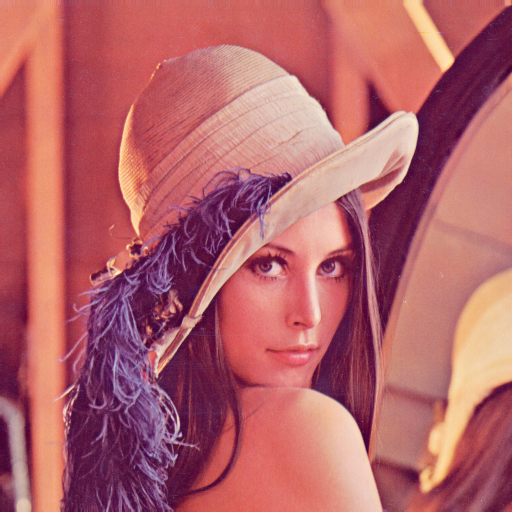
\includegraphics[width=7cm]{image-blur/lenna.png}}}
    \qquad
    \subfloat[\centering Lenna Image with Motion Blur] {{\includegraphics[width=7cm]{image-blur/lenna-motion-blur.png}}}
    \qquad
    \subfloat[\centering Lenna Image with Radial Blur] {{\includegraphics[width=7cm]{image-blur/lenna-radial-blur.png}}}
    \qquad
    \subfloat[\centering Lenna Image with Gaussian Blur $\sigma = 0.85$] {{\includegraphics[width=7cm]{image-blur/lenna-gaussian.png}}}
    \caption{\centering Different Blurs applied to the Lenna Image \label{fig:lenna-blur}}
\end{figure}

\clearpage
\section{Blind Image Deblurring Methods}
Image deblurring is a process of recovering the original image from a degraded image degraded by blur. There are two types of image deblurring, first is the blind image deblurring and second is the non blind image deblurring. Blind image deblurring is a process of deconvolution in which both the actual image and the degradation function is unknown and only the degraded image is known. In this thesis we discuss two blind deblurring methods. 

\begin{enumerate}
    \item Maximum a posterior based method 
    \item Eigen value based method 
\end{enumerate}

\subsection{Blind Deconvolution Using Maximum a Posteriori} \cite{24}
This is a single image blind deconvolution method. Its goal is to estimate the unknown degradation function (blur) from a single blurred image and reconstruct the original sharp image. Such task is ill posed and involves some heuristic or other steps to arrive at a desired solution. Here we show that a very straightforward maximum a posteriori method included with very sparse priors and an efficient numerical solving method can produce good results, which can compete with much more  complex and complicated state-of-the-art methods. \\

We rewrite the equation showing blur degrading model: \\

\begin{equation*}
    b = i * h + \eta
\end{equation*}

where $b$ is the blurred image, $u$ is the sharp image(unknown), $h$ is known as the point spread function (PSF) (unknown) and $\eta$ is random additive noise. Now we have only one observation i.e. one blurred image and no knowledge of the PSF, thus the problem is extremely ill-posed. A lot of effort has been made in the field of image processing by the researcher community in the last few decades to find a reliable algorithm for blind deblurring or mathematically deconvolution with general PSFs. First algorithm in blind image deconvolution appeared in the field of telecommunication and signal processing in early 80’s \cite{6}. Proposed algorithms worked only for special cases of applications, such as where blurring was due to symmetric PSFs or astronomical images which had uniform black background. \\

When we see the problem from probabilistic point of view  recovery of u and h iteratively equates to solving MAP (Maximum A Posteriori) estimation. 

\begin{equation}
    P(i \cdot h | b) \propto P(b | i \cdot h) P(i, h) = P(b | i \cdot h) P(i) P(h)
\end{equation}

where $P(g | u \cdot h) \propto \exp{-\frac{\gamma}{2} \|i * h - b\|^2}$ is the noise distribution of the image (in this case assumed Gaussian) and $P(i)$, $P(h)$ are the prior distributions of the true image and blur kernel (PSF), respectively. \\

The main idea of this algorithm is to solve the ill-posedness of blind deconvolution by characterizing the prior $P(i)$ by using statistics of the natural images and by correct choice of estimators.  

\subsubsection{Mathematical Model}
Lets assume that the individual variables used in the blur degradation model are discrete quantities which are indexed and denoted as $u_i$ or $[u]_i$. Maximization of the posterior probability $P(i,h | b)$ is equivalent to the minimization of the negative logarithm of it, i.e.

\begin{equation}
    L(i, h) = -\log{P(i, h | b)} + const = \frac{\gamma}{2} \|i * h - b\|^2 + Q(i) + R(h) + const
\end{equation}

where $Q(i) = −\log{P(i)}$ and $R(h) = −\log{P(h)}$ are regarded as regularizers that track the optimization to the correct result and away from infinite number of other wrong and unwanted solutions. \\

The most popular choice of researches is probably the $l_1$ norm of the derivatives of the images which is either directionally separable $Q(i) = \sum |D_x(i) + D_y(i)|$ (this  is the Laplace distribution of image derivatives) or isotropic (in terms of image gradient) $Q(i) = \sum |D_x^2(i) + D_y^2(i)|$ where $D_x$ and $D_y$ are partially derivative operators. It has been found that the distribution of gradients found from natural images is more heavy tailed than laplace distribution thus we use a generic version of $Q(i)$ defined as

\begin{equation}
    Q(i) = \sum |D_x^2(i) + D_y^2(i)|^ {p/2} \hspace{.5cm} 0 \leq p \leq 1
\end{equation}

In the case of blur kernel to force sparsity and zero for the negative values we use Laplace distribution on the positive values of the kernel. This results in the following regularizer R is thus defined as: 

\begin{align}
    R(h) &= \Psi(h_i) \\
    h_i &= \begin{cases}
        hi & h_i > 0 \\
        0  & h_i < 0
    \end{cases}
\end{align}

\subsubsection{Optimization Algorithm}
To find out numerically the solution of i, h we minimize the functional L in alternately with respect to i and h and at the same time keeping the other quantities constant. For minimization of each sub problem we use  augmented Lagrangian method (ALM). \\

\textbf{5.1.2.1 Minimization with Respect to $i$} \\

The equation which needs to be computed for estimation of $i$ is

\begin{equation}
    \min\limit_{i}{\frac{\gamma}{2} \|i * h - b\|^2 + \Phi(v_x, v_y)}
\end{equation}

where $v_x = D_xi$ and $v_y = D_yi$, ALM optimization algorithm adds a penalty term which is quadratic for each constraint to the traditional Lagrangian method, 

\begin{equation}
    L(i, h) = \frac{\gamma}{2} \|i* h - b\|^2 + \frac{\alpha}{2} \|D_xi - v_x - a_x\|^2 + \frac{\alpha}{2} \|D_yi - v_y - a_y\|^2
\end{equation}

where $a_x$, $a_y$ are the new variables in the equation which are proportional to the Lagrange multipliers of the constraints. After such reformulation, the data term (1st term in the equation)  and the regularizer $\Phi(v_x, v_y)$ can be considered two minimization problems as they depend on different variables and are minimized separately. By introducing the penalty terms by ALM, it allows us to deal with the constrained variables $D_xu$ and $v_x$ (similarly $D_yu$ and $v_y$) as they were unrelated and by taking the penalty weight α sufficiently large, we are able to obtain the solution for the main problem. \\

We solve the problem of minimization of $L(i)$ to obtain $i$, $v_x$, $v_y$ we compute the derivative of $L$ with respect to one variable while keeping others fixed. Then we solve it for minimum value of $L(i)$ and update that variable based on that. Finally we move on to the next variable and again follow the same process. This process is done iteratively for much iteration. After the process of differentiating $L(i)$ w.r.t. $i$ and equating the derivative to zero, we must solve the linear system  for $i$. Thus, the solution for $i$ can be easily computed and only by using the very famous Fourier transform. \\

Minimization of $L_i$ w.r.t. $v_x$, $v_y$ on is a bit trickier to calculate. For minimization of $v_x$ and $v_y$ the function to minimize is given by: 

\begin{equation}
    \Phi(v_x, v_y) + \frac{\alpha}{2} \|D_xi - v_x - a_x\|^2 + \frac{\alpha}{2} \|D_yi - v_y - a_y\|^2
\end{equation}

Derivatives and minimization of the above equation can therefore carried out pixel by pixel independently.  Let $t = (v_xi, v_yi)$ and $w = (D_xu(i) − a_xi, D_yu(i) − a_yi)$, then the equation available for minimizing Li  w.r.t. [vx]i, [vy]i can be rewritten as

\begin{equation}
    \min\limit_{t} \|t\|^q + \frac{\alpha}{2} \|t - w\|^2
\end{equation}

For some value of $q$ a solution can be computed. If we do some simple calculation then it can be found that for the generic choice of $q = 1$, \\

\textbf{5.1.2.2 Minimization With Respect To $h$} \\

Minimizing of the likelihood function can be done with respect to h and the solution to it can be found in a similar fashion. In the similar way to separate the minimization of data term and regularizer, we again make the substitution $v_h = h$. So this can be visualized as the following optimization problem. \\

\begin{equation}
    \min\limit_{h} \frac{\gamma}{2} \|i * h - b\|^2 + R(v_h) \hspace{.4cm} \text{where $v_h = h$}
\end{equation}

Now again we apply Augmented Lagrangian Method (ALM) and the optimization equation becomes

\begin{equation}
    \frac{\gamma}{2} \|i * h - b\|^2 + R(v_h) + \frac{\beta}{2} \|h - v_h - a_h\|^2
\end{equation}

where $a_h$ is again similar to the variable introduced in the last sub-section related to ALM method and also  proportional to the constraint’s Lagrange multiplier. Minimization of the above equation w.r.t. $v_h$ can be done again component-wise like the last sub-section. Here $t = v_h \cdot i$, $w = (h − a_h) \cdot i$, \\

then the problem can be rewritten as 

\begin{equation}
    \min\limit_{t} \frac{\beta}{2} \|w - t\|^2 + \Psi(t)
\end{equation}

which is basically for p = 1 with the additional constraint that t has only positive values. 

\begin{figure}
    \centering
    \includegraphics{blind-image-deblurring-methods/results.PNG}
    \caption{Results of MAP Based De-Blurring}
    \label{fig:results}
\end{figure}

\subsection{Blind Image Deblurring Using Eigen Value/Vector}
Blind image deconvolution is a process to recover a sharp image version of a known blurry image when the degradation function or blur kernel or psf is unknown. \cite{25} This problem is ill conditioned by nature and effectual criteria for both the sharp image and blur kernel is needed to properly constrain the space of problem solutions. The problem of blind image deconvolution has been extensively studied for very long but it is still not clear how to correctly regularize the blur kernel.  \\

The concept of deblurring that is explained in this section is based on assumption that the blurry image actually has inside rich information about the degradation function/blur kernel, and such type of information can be found by finding and utilizing a very well known phenomenon stated that sharp images are often high pass i.e. contain high frequency information whereas blurry images are usually low pass i.e. they contain low frequency information. \\

The equation showing blur can be written as, 

\begin{equation}
    B \approx I_0 * H_0
\end{equation}

Where $B$ is the blurred image, $I_0$ is the blur free image, $H_0$ is the blur kernel and $*$ denotes the discrete convolution operator. $(n_1, n_2)$ is the size of the image, and $(m_1, m_2)$ is the size of the blur kernel. The blind image deblurring problem is mathematically expressed as the problem of blind deconvolution, which is to recover the sharp image $I_0$ when the degradation function/blur kernel $H_0$ is unknown. \\

A direct approach for blind deconvolution is to subsequently determine the true image $I_0$ and the blur kernel $H_0$ by 

\begin{equation}
    \min\limit_{I_0, H_0} \|B - I_0 * H_0\|^2
\end{equation}

The bad thing is that the above optimization is severely ill-posed, because it can be minimized exactly by infinite number of  $(I, H)$ pairs. For example,  $(I = B, K = δ)$ is also a perfect solution, because $B = B * \delta$ where $\delta$ is delta kernel. So generally it becomes necessary to regularize the required solution for the image $I$.

\begin{equation}
    \min\limit_{I, H} \|B - I * H\|^2 + \lambda f(I)
\end{equation}

where $\lambda \geq 0$ and $f(I)$ ia a regularizer which is generally chosen as the total variation or its variations. But this still has the $B$, $\delta$ solution. Hence, it is also important and in fact unavoidable to regularize the blur kernel $H$, i.e., it is necessary to consider an extension.

\begin{equation}
    \min\limit_{I, H} \|B - I * H\|^2 + \lambda f(I) + a \cdot h(H)
\end{equation}

where $\lambda \geq 0$ and $\alpha \geq 0$. $h(K)$ can be different regularizers like the sparse regularizer $h(K)=\|K\|_1$ , Gaussian function $h(K) =\|K\|_F$  the and the Bayesian prior. We show a regularizer which is more effective for the blur kernel that can significantly benefit the required solution of the blind deconvolution/deblurring problem. This regularizer is based on an observation which is well known in all matter that blurry images are usually having low pass information and sharp images are having high-pass information. Blurring reduces the high frequency components of the true blur free image. The idea is to exploit the spectral properties of the blurred/blur free image as a convolution operator. \\

For a given image which is a matrix we consider its convolution with any known/unknown matrix. The convolution operator is a linear operator. The classical knowledge shows that the spectrum ( fourier frequencies) of the linear operator of a blurry image should be much smaller than that for the blur free image.  Even if the image is blurred such that human eyes cannot recognize the details in it, it is still possible to restore a sharp version with sharp details by recovering the blur kernel. \\

The regularizer $h^{L(B)}(H)$ depends on the degraded blurry image and has lot of information about the relation between blurry image $B$ and the sharp image $I_0$. Hence it is natural to guess that this type of regularizer $h^{L(B)}(H)$ would depend on the true sharp image $I_0$ also. But surprisingly, under a variety of  conditions, the derived regularizer $h^{L(B)}(H)$ can come up in a very effective manner and it does not depend on the information of the true sharp image $I_0$. Thus the desired kernel (blur) $H_0$ can be retrieved successfully. \\

It is very well known that there are many (infinite) number of ways to decompose the degraded blurry image $B$ into the relation based on convolution of $I$ and $H$. The frequency spectrum of the images in the edge domain is more hampered by blurring than in the actual pixel domain. Thus the degradation function or blur kernel H0 is restored by the edge features rather than the raw (actual) pixel values.  

\subsubsection{Blind Deblurring by Spectral Properties}
In sub section a rigorous derivation that explains how the proposed regularizer $h^{L(B)}(K)$ is established is presented. \\

\textbf{5.2.1.1 Spectrum of an Image as a Convolution Operator} \\

The operation and application of convolution is well known. But I would briefly show it mathematically. Suppose A and B are functions are represented by matrices. Then the convolution procedure of A and B can be written as  

\begin{equation}
    (A * B)(i, j) = \sum\limit_{i, j} A(i - u, j - v) B(u, v)
\end{equation}

Convolution is a linear operator and can be easily converted into a format of matrix multiplication. Let $v (\cdot)$ be the matrix vectorization. Then it can be manipulated that 

\begin{equation}
    v(X * Y) = A_{k_1, k_2}(X) \cdot v(Y)
\end{equation}

where $A_{k_1, k_2} (\cdot)$ is the convolution matrix of the variable and $k_1, k_2$ are taken kernel size. For an image with size $(l_1, l_2)$ i.e. matrix $X$ here, it is a convolution matrix, denoted by $A_{k_1, k_2}(X)$. The size of the convolution matrix  is  $((l_1 + k_1 − 1)(l2 + k2 − 1), k_1 \cdok k_2)$.  \\

\textbf{5.2.1.2 Convolution Eigen values/vectors} \\

Image $I$ is operated as a matrix related with a certain feature filter $L$.

\begin{equation}
    L(I) = L * I
\end{equation}

We can choose any feature filter for L but we have used L as a Laplacian of Gaussian (LoG) which means we are using edge features.  \\

For any image $I$ which is presented by a feature filter $L$ as discussed above its very first convolution eigenvalue written as $\sigma^{L}(I)$ as defined as

\begin{equation}
    \sigma^{L}(I) = \max \|l(I) * X\|_{F}^2 \hspace{.4cm} \text{where $\|X\|_F = 1$}
\end{equation}

The value of X for which the above problem maximizes is called as the first convolution eigenvector, denoted as $k_1^L(I)$. Similarly other eigen values can also be defined in terms of the eigen vectors. 

\begin{equation}
    \sigma_i^L(I) = \max \|L(I) * X\|^2_F
\end{equation}

The classical Fourier theory tells that the eigen values of a given image tells about the frequency components of the image and are indeed linked to the frequency components present in the image. It can be clearly seen that the eigen vectors and eigen values are the right singular vectors/values of the convolution matrix. So, for a given image I which has the convolution matrix $A_{s_1, s_2}(L(I))$ all its convolution eigenvalues and eigenvectors can be found by applying Singular Value Decomposition (SVD) of the matrix, square to convolution matrix. \\

It has been discussed that the degraded blurry images generally contains low frequency information and the sharp images often contain high frequency information, so we can say that blurring decreases dramatically the Fourier frequencies of a sharp image. In other words, blurring process can majorly reduce the eigen values, which show the image’s frequencies in frequency domain. \\

Thus we can say that 

\begin{equation}
    \sigma^{L}(B) \leq \sigma^{L}(I)
\end{equation}

An image $I$ is checked for blur and called $\tau$-sharp if $\sigma^L(I) \geq \tau$  where $\tau > 0$. In general, the convolution eigen values of true sharp images are very large as compared those of blurry images which are much smaller. \\

\textbf{5.2.1.3 PSF Regularizer} \\

By making use of the observation discussed above that blurring of images could significantly decrease the frequencies present in the image or we can also say the decrease in  the convolution eigen values, we can derive a regularizer, denoted as $h^{L(B)}(H)$. The interesting part is that this regularizer tends to get minimized at the desired (actual) blur kernel (psf), $H_0$. \\

We begin with a very simple situation where the degraded blurry image $B$ is produced by the linear convolution of $I_0$ and $H_0$ i.e., $B = I_0 * H_0$. When we work in the edge domain then the equation becomes

\begin{equation}
    L(B) = L(I_0) * L(H_0)
\end{equation}

where $L$ is choosen as laplacian of Gaussian (LoG), i.e., we use edge features. 

\begin{align}
    \sigma_i^L(B) &= \|L(I_0 * H_0) * k_i^L(B)\|^2_F \\
    \frac{\sigma_i^L(B)}{H_0 * k_i^L(B)} &= \norm{L(I_0) * \frac{H_0 * k_i^L(B)}{H_0 * k_i^L(B)}} 
\end{align}

Thus we have

\begin{equation}
    \frac{\sigma_i^L(B)}{\sigma_{\min}^L(I_0)} \geq H_0 * k_i^L(B)
\end{equation}

Now next check the lower convolution eigenvectors of the degraded blurry image $B$ i.e., the  eigenvectors which belong to the low frequency components of $B$. Due to the known fact that the true image $I_0$ is high pass information and has a very large $\sigma_{\min}^L(I_0)$ the ratio in the above equation should be very small. \\

So now we define the regularizer as 

\begin{equation}
    h^{L(B)}(H_0) = \mathlarger{\mathlarger{\sum\limit_{i=1}^{s_1, s_2}}} \frac{\norm{H_0 * k_i^L(B)}^2}{\sigma_i^L(B)^2}
\end{equation}

The weight $1 / \sigma_i^L(B)^2$ drops rapidly when $\sigma_i^L(B)^2$ goes bigger and numerator of the above equation corresponding to small convolution eigen values will lead the function. On minimizing this equation we can recover the blur kernel Ho without using any information of $I_0$ the true sharp image. 

\begin{equation}
    \hat{H_0} = \min\limit_{H_0} h^{L(B)}(H)
\end{equation}

\subsubsection{Image Deconvolution}

Now we know the blur kernel and thus we can proceed with the image deconvolution for the extraction of the true sharp image from the degraded blurred image. The deconvolution of the blurred image involves the minimization of the below given equation. 

\begin{equation}
    \min\limit_{I, H} \norm{B - I * H}^2 + \lambda \norm{\nabla I}_1 f(I) + a h^{L(B)}(H)
\end{equation}

The process of minimization goes in two steps: 

\begin{enumerate}
    \item Minimization of the optimization equation knowing the blur kernel $H$ for expected true image $I$. 
    \item Minimization of the optimization equation for the blur kernel using the estimated true sharp image in the last step. 
\end{enumerate}

This process is repeated hundreds of times in an iterative manner and finally we get the true sharp image and the degradation function also called blur kernel. 

\begin{figure}[ht]
    \centering
    \includegraphics{blind-image-deblurring-methods/eigen-based.PNG}
    \caption{Eigen Based Image Deblurring Results}
    \label{fig:eigen-based}
\end{figure}

\clearpage
\section{Proposed Method}
Blind image deconvolution is a process to recover a sharp image version of a known blurry image when the degradation function or blur kernel or psf is unknown. This problem is ill conditioned by nature and effectual criteria for both the sharp image and blur kernel is needed to properly constrain the space of problem solutions. The problem of blind image deconvolution has been extensively studied for very long but it is still not clear how to correctly regularize the blur kernel. \\

The concept of deblurring that is explained in this section is based on assumption that the blurry image actually has inside rich information about the degradation function/blur kernel, and such type of information can be found by finding and utilizing a very well known phenomenon stated that sharp images are often high pass i.e. contain high frequency information whereas blurry images are usually low pass i.e. they contain low frequency information and by utilizing the Bayesian approach of maximum a posterior.  \\

The equation showing blur can be written as

\begin{equation}
    B \approx I_0 * H_0
\end{equation}

Where $B$ is the blurred image, $I_0$ is the blur free image, $H_0$ is the blur kernel and $*$ denotes the discrete convolution operator. $(n_1, n_2)$ is the size of the image, and $(m_1, m_2$ is the size of the blur kernel. The blind image deblurring problem is mathematically expressed as the problem of blind deconvolution, which is to recover the sharp image $I_0$ when the degradation function/blur kernel $H_0$ is unknown. \\

A direct approach for blind deconvolution is to subsequently determine the true image $I_0$ and the blur kernel $H_0$ by

\begin{equation}
    \min\limit_{I_0, H_0} \norm{B - I_0 * H_0}^2
\end{equation}

Now we explain the proposed method for the process of image deconvolution. We first use the maximum a posterior method to solve the optimization problem. The relation between the blurred image, sharp image and the degradation function in terms of probability is 

\begin{equation}
    P(i, h | b) \propto P(b | i, h) P(i, h) = P(b | i, h) P(i) P(h)
\end{equation}

Maximization of the posterior probability $P(i,h | b)$ is equivalent to the minimization of the negative logarithm of it, i.e., 

\begin{equation}
    L(i, h) = -\log{P(i, h | b)} + c = \frac{\gamma}{2} \norm{i * h - b}^2 + Q(i) + R(h) + c
\end{equation}

where $Q(i) = −\log{P(i)}$ and $R(h) = −\log{P(h)}$ are regarded as regularizers that track the optimization to the correct result and away from infinite number of multiple incorrect and unwanted solutions. \\

By solving this for $I$ and $H$ we get an estimate of the true sharp image but the image is still not fully blur free so something else needs to be done to remove it. \\

So now we take the estimate of the true sharp image is taken as the blurred image and we use the eigen value based method to solve the problem in hand. We find the blur kernel by minimizing the equation for Ho given by 

\begin{equation}
    h^{L(B)}(H_0) = \mathlarger{\mathlarger{\sum\limit_{i = 1}^{s_1, s_2}}} \frac{\norm{H_0 * k_i^L(B)}^2}{\sigma_i^L(B)^2}
\end{equation}

Further when we have calculated the blur kernel then we iteratively minimize the given equation to finally find the true sharp image using 

\begin{equation}
    \min\limit_{I, H} \norm{B - I * H}^2 + \lambda \norm{\nabla I}_1 f(I) + a h^{L(B)}(H)
\end{equation}

\begin{figure}
    \centering
    \includegraphics{proposed-method/result-final.PNG}
    \caption{Final Results Using The Proposed Method}
    \label{fig:my_label}
\end{figure}

\clearpage
\begin{thebibliography}{9}

\bibitem{gonzalez-woods}
\href{https://www.pearson.com/us/higher-education/program/Gonzalez-Digital-Image-Processing-4th-Edition/PGM241219.html}{Gonzalez C.Rafeal,Woods Richard E., ”Digital Image Processing”, London Pearson Education, 2002. }

\bibitem{jain-anil}
\href{https://dl.acm.org/doi/book/10.5555/59921}{Jain Anil K.,”Fundamentals of Digital Image Processing”, Davis:Prentice-Hall of India, 2000.}

\bibitem{jiang-ming}
\href{https://www.ijccer.org/index.php/ojs/article/view/115}{Jiang Ming,Wang Ge,”Development of blind image deconvolution and its application”, Journal of X-Ray Science and Technology,IOS Press,11(2003),pp. 13-19.  }

\bibitem{chang-mm}
\href{https://baixardoc.com/documents/digital-image-processing-4th-edition-william-k-pratt-edwara--5d0a9c64c59cd}{Chang M.M., Tekalp A.M., and Erdem A.T., ”Blur identification using the bispectrum,”IEEE Trans Signal Processing, vol.39(10), October 1991, pp.2323-2325. Ayers G.R., Dainty J.C., ”Iterative Blind Deconvolution method and its application”, Optics Letter,vol.13(7), July 1988, pp.547-549.}

\bibitem{5}
\href{https://www.academia.edu/8030569/DEBLURRING_OF_IMAGES_USING_BLIND_SCHEMES}{Biretta J., ” WFPC and WFPCC 2 Instrumental Characteristics,in the Restoration of HST images and Spectra-2”, Space Telescope Science Institute, Baltimore, MD,1994, pp.224-235. }

\bibitem{6}
\href{https://www.ima.umn.edu/materials/2005-2006/MM8.9-18.06/1590/team5_rep.pdf}{Krahmer Felix, Lin Youzuo,McAdoo Bonnie,Ott Katharine,Wang David, Widemann Jiakou, ”BLIND IMAGE DECONVOLUTION:MOTION BLUR ESTIMATION”, Aug 18(2006).}

\bibitem{7}
\href{https://www.academia.edu/8030569/DEBLURRING_OF_IMAGES_USING_BLIND_SCHEMES}{Tan Wenzhao, Zhang Jin, Rong Gang, Chen Huirnng, ”Identification of Motion Blur Direction Based on Analysis of Intentional Restoration Errors”, Proceedings of 2004 IEEE, March 21-23(2004), pp 1253-1258. }

\bibitem{8}
\href{https://www.academia.edu/8030569/DEBLURRING_OF_IMAGES_USING_BLIND_SCHEMES}{Stern A., Kopeika N.S., ”Analytical method to calculate optical transfer functions for image motions and vibrations using moments”, Optical Society of America, vol 14(2), February 1997, pp.388-396.}

\bibitem{9}
\href{https://ieeexplore.ieee.org/document/6497608}{Mariana S. C. Almeida and Mário A. T. Figueiredo, “Parameter Estimation for Blind and Non-Blind Deblurring Using Residual Whiteness Measures”, IEEE TRANSACTIONS ON IMAGE PROCESSING, VOL. 22, NO. 7, JULY 2013 }

\bibitem{10}
\href{https://ieeexplore.ieee.org/abstract/document/6805611/}{Tao Yue, Jinli Suo, and Qionghai Dai, “High-Dimensional Camera Shake Removal With Given Depth Map”, IEEE TRANSACTIONS ON IMAGE PROCESSING, VOL. 23, NO. 6, JUNE 2014}

\bibitem{11}
\href{https://ieeexplore.ieee.org/iel7/83/6587532/06497606.pdf}{C. S. Vijay, C. Paramanand, A. N. Rajagopalan, and Rama Chellappa,” Non-Uniform Deblurring in HDR Image Reconstruction”, IEEE TRANSACTIONS ON IMAGE PROCESSING, VOL. 22, NO. 10, OCTOBER 2013 }

\bibitem{12}
\href{https://ieeexplore.ieee.org/document/6915685}{Alexandra Nasonova and Andrey Krylov,” Deblurred Images Post-Processing by Poisson Warping”, IEEE SIGNAL PROCESSING LETTERS, VOL. 22, NO. 4, APRIL 2015}

\bibitem{13}
\href{https://ieeexplore.ieee.org/document/5445028}{Manya V. Afonso, Jose M. Bioucas-Dias and Mario A. T. Figueiredo,” Fast Image Recovery Using Variable Splitting and Constrained Optimization”, IEEE TRANSACTIONS ON IMAGE PROCESSING, 2010 }

\bibitem{14}
\href{https://citeseerx.ist.psu.edu/viewdoc/download?doi=10.1.1.329.7593&rep=rep1&type=pdf}{WIKKY FAWWAZ A M, TAKUYA SHIMAHASHI, MITSURU MATSUBARA, and SUEO SUGIMOTO,” PSF Estimation and Image Restoration for Noiseless Motion Blurred Images”, International Conference on Signal, Speech and Image Processing, Beijing, China, September 15-17, 2007}

\bibitem{15}
\href{https://link.springer.com/article/10.1186/1687-6180-2012-3}{Hae-Jong Seo and Peyman Milanfar,” Robust flash denoising/deblurring by iterative guided filtering”, EURASIP Journal on Advances in Signal Processing 2012}

\bibitem{16}
\href{https://www.semanticscholar.org/paper/Estimation-and-Removal-of-Motion-Blur-by-Capturing-Lim-Silverstein/a598119ba16805c63f227bf4252793686f190182}{Suk Hwan Lim, Amnon Silverstein.” Estimation and Removal of Motion Blur by Capturing Two Images with Different Exposures”, HP Laboratories HPL-2008-170}

\bibitem{17}
\href{https://www.ijcaonline.org/archives/volume72/number17/12634-9228}{Kishore R. Bhagat and Puran Gour,”Novel Approach to Estimate Motion Blur Kernel Parameters and Comparative Study of Restoration Techniques”, International Journal of Computer Applications (0975 – 8887) Volume 72– No.17, June 2013}

\bibitem{18}
\href{https://ci.nii.ac.jp/naid/10003556726/}{\textbf{MATLAB}: "Computer Methods For Mathematical Computations" Cleve Moler}

\bibitem{19}
\href{}{Deveneder Sharma, Puneet Sharma, Ritu Sharma \textbf{Comparative Analysis of Various Techniques for Non-Blind Restoration of Images} International Journal of Advanced Research in Computer and Communication Engineering Vol. 2, Issue 8, August 2013}

\bibitem{20}
\href{mdpi.com/1424-8220/8/9/6108/html}{Amar A. El-Sallam and Farid Boussaid \textbf{Spectral-Based Blind Image Restoration Method for Thin TOMBO Imagers}}

\bibitem{21}
\href{https://ieeexplore.ieee.org/document/5760166}{S. Ramya; T. Mercy Christial \textbf{Restoration of blurred images using Blind Deconvolution Algorithm}  2011 International Conference on Emerging Trends in Electrical and Computer Technology}

\bibitem{22}
\href{https://www.ijireeice.com/upload/2016/december-16/IJIREEICE\%2011.pdf}{Chandra Prakash Prabhakar, Mrs. Kiran Dewangan \textbf{Estimation of Motion Blur Based on
Combination of PSO and GA} International Journal of Innovative Research in
Electrical, Electronics, Instrumentation and Control Engineering}

% 11
\bibitem{23}
\href{https://www.sciencedirect.com/science/article/abs/pii/S0378475417302793?via\%3Dihub}{Skander Belhaj, Haithem Ben, Kahla, Marwa Dridi, Maher Moakher \textbf{Blind image deconvolution via Hankel based method for computing the GCD of polynomials} Elsevier}

% 3 
\bibitem{24}
\href{https://link.springer.com/book/10.1007\%2F978-3-642-40246-3}{Springer \textbf{Computer Analysis of Images and Patterns} 15th International Conference, CAIP 2013, York, UK, August 27-29, 2013, Proceedings, Part II}

% 2 
\bibitem{25}
\href{https://ieeexplore.ieee.org/document/6918507}{Guangcan Liu, Shiyu Chang, Yi Ma et al. \textbf{Blind Image Deblurring Using Spectral Properties of Convolution Operator} IEEE Transactions on Image Processing ( Volume: 23, Issue: 12, Dec. 2014)}

\end{thebibliography}
\end{document}
